%% $RCSfile: proj_proposal.tex,v $
%% $Revision: 1.2 $
%% $Date: 2010/04/23 02:40:16 $
%% $Author: kevin $

%\documentclass[11pt, a4paper, twoside, openright]{report}
\documentclass[12pt, a4paper, openright]{report}
\usepackage{float} % lets you have non-floating floats
\usepackage{graphicx}
\usepackage{url} % for typesetting urls
\usepackage[nottoc,notlof,notlot]{tocbibind} 
\usepackage{algorithm2e}
\renewcommand\bibname{References}
\usepackage{amsmath,amssymb,amsthm,mathrsfs,amsfonts,dsfont}
%  We don't want figures to float so we define
%
\newfloat{fig}{thp}{lof}[section]
\floatname{fig}{Figure}
\renewcommand*\contentsname{Table Of Contens}
%% These are standard LaTeX definitions for the document
%%


\title{Kickoff, A Tool For Software Companies To Control Their Labor Cost Safely}
\author{Zhu Yue Cai}


%% This file can be used for creating a wide range of reports
%%  across various Schools
%%
%% Set up some things, mostly for the front page, for your specific document
%
% Current options are:
% [ecs|msor]              Which school you are in.
%
% [bschonscomp|mcompsci]  Which degree you are doing
%                          You can also specify any other degree by name
%                          (see below)
% [font|image]            Use a font or an image for the VUW logo
%                          The font option will only work on ECS systems
%
\usepackage[font]{vuwproject} 

% You should specifiy your supervisor here with
    \supervisor{Dr. Brandiff Caron}
    %\authorAddress{3305 De Rouen, Montreal}
% use \supervisors if there are more than one supervisor

% Unless you've used the bschonscomp or mcompsci
%  options above use
%   \otherdegree{OTHER DEGREE OR DIPLOMA NAME}
% here to specify degree

% Comment this out if you want the date printed.
\date{}
\pagenumbering{alph}
\begin{document}

% Make the page numbering roman, until after the contents, etc.
\frontmatter

%%%%%%%%%%%%%%%%%%%%%%%%%%%%%%%%%%%%%%%%%%%%%%%%%%%%%%%

\begin{abstract}
	
	\addcontentsline{toc}{chapter}{Cover Page}
  This document gives some ideas about how to write a project
  proposal, and provides a template for a proposal. You should discuss
  your proposal with your supervisor.
\end{abstract}

%%%%%%%%%%%%%%%%%%%%%%%%%%%%%%%%%%%%%%%%%%%%%%%%%%%%%%%

\maketitle
%\pagestyle{empty} %get rid of header/footer for toc page
\tableofcontents %put toc in
%\cleardoublepage %start new page
%\pagestyle{plain} % put headers/footers back on
\setcounter{page}{2} %reset the page counter
\addcontentsline{toc}{chapter}{Table of Contents}
\chapter*{Executive Summary}
%\addcontentsline{toc}{chapter}{Letter of Transmittal}
\setcounter{page}{3}
\addcontentsline{toc}{chapter}{Executive Summary}

% we want a list of the figures we defined


%%%%%%%%%%%%%%%%%%%%%%%%%%%%%%%%%%%%%%%%%%%%%%%%%%%%%%%

\mainmatter

%%%%%%%%%%%%%%%%%%%%%%%%%%%%%%%%%%%%%%%%%%%%%%%%%%%%%%%

%\listof{fig}{LIST OF FIGURE}
%\addcontentsline{toc}{chapter}{LIST OF FIGURE}

\chapter*{}
%\section* {1. Body of Proposal}
%\addcontentsline{toc}{chapter}{1. Body of Proposal}

\section*{1. INTRODUCTION}
\addcontentsline{toc}{chapter}{1. INTRODUCTION}
Laying off developers and recruiting new joiners are two common software company activities. But Previous research has shown that high turnover rates leads to a decrease in productivity \cite{Guthrie2001AMJ}. 
Like other jobs that involve knowledge workers, 
when a software developer leaves, there is a knowledge gap. This gap is manifested as abandoned
files on the software system that can be difficult to maintain.


Generally, these abandoned files are taken over by new joiners or remain developers. There is a large literature on mentoring and integrating new developers into software projects. For example, Zhou and Mockus examined the impact of development environment on new developers\cite{Zhou2011ICSE} . Bird et al. \cite{Bird2007MSR} looked at the survival rate of new developers. Zhou and Mockus examined the amount of time until a developer becomes productive. Mockus \cite{Mockus2010FSE} suggested mentors for developers based on past work and Canfora et al. \cite{Canfora2012FSE} suggested mentors based on the email communication network. The experienced developers who have the knowledge to the abandoned files will help reduce the damage. They can take over the abandoned files themselves or mentor the new joiner to do so.


Therefore We believe that a software which can calculate the number of abandoned files and produce a list of experienced  developers who have the knowledge to those files for a given layoff list is very helpful. Moreover, If this software could tell the same information for all the possible 
layoff lists based on input critical variables, the decision process would be simplified dramatically. This is the motivation of Kickoff. It is a useful management tool for software company to manage its knowledge storage.



\newpage
\section*{2. METHODOLOGY}
\addcontentsline{toc}{chapter}{2. METHODOLOGY}

In order to minimize the cost, we will use only opensource tool to build Kickoff. And what we need is "PostgreSQL"as our database.

In computer software engineering, revision control, or version control, is any kind of practice that tracks and provides control over changes to source code. Software companies use version control software to maintain documentation and configuration files as well as source code.
The first step of building Kickoff is to develop a mechanism to extract the source code change history from their version control software. Nowadays, a large number of software companies use "Git" as their version control system which is also opensource. Therefore "Kickoff" should be able to extract information from "Git" at the beginning. Since "Git" has a function called blame can identify changes and who made the changes in your project, we only need to input the result in the database. And this can be done by string processing technique and the psql command. We only need to integrate this into the software.    

With the database ready, It is easy to calculate the number of abandoned files for a single given layoff list or for all possible lists of a given size. But it is very difficult to calculate the number for all potential layoff lists. 
We can use the "truck factor" algorithm proposed by Ricca et el \cite{Ricca2011PROFES} for the job. In software development, the truck factor is the number of key developers who would need to be incapacitated to make a project unable to proceed. It is also known as bus factor, or lottery factor and is a measurement of the concentration of information in individual team members. The concept of truck factor is not related to the project, but the algorithm to calculate it is what we need. However, as Ricca et el pointed out\cite{Ricca2011PROFES}, the time complexity of this algorithm is too large to implement in the industry. Therefore, optimizing this algorithm is the first problem we need to solved. We introduced a stopping condition to optimize the naive algorithm. What it does is to determine whether the unarticulated lists will have a number of abandoned files greater than the input value. If no, it will stop the program and save time. Then with the user input their maximum acceptable abandoned files amount, The program will work only for the layoff lists that satisfies the condition. For more detail about the optimized truck factor algorithm, please refer to Appendix A.  


Even with this optimization, the algorithm is only piratical to company with less than 100 developers. Further research on how to apply parallel computing technique in the optimized truck factor algorithm is required, such that it is also piratical large software companies.


The second problem is how to integrate previous researches to generate an algorithm for selecting the experienced developers for each abandoned file. We introduce a successor candidate selecting algorithm for this functionality. The general idea of this algorithm is to pick out those developers who have worked with the files that have co-changes with the abandoned files as candidates. The intuition behind is that if file A has changed with file B, and file A becomes abandoned, then the developer who works on file B will likely know something about file A. The idea of this algorithm comes from the matrix multiplication in Cataldo et al.'s\cite{Cataldo2006CSCW}


With all these function units prepared, the conceptual structure of Kickoff is shown in the following figure\ref{structure}.
\DeclareGraphicsExtensions{.pdf,.png,.jpg}
\begin{center}
	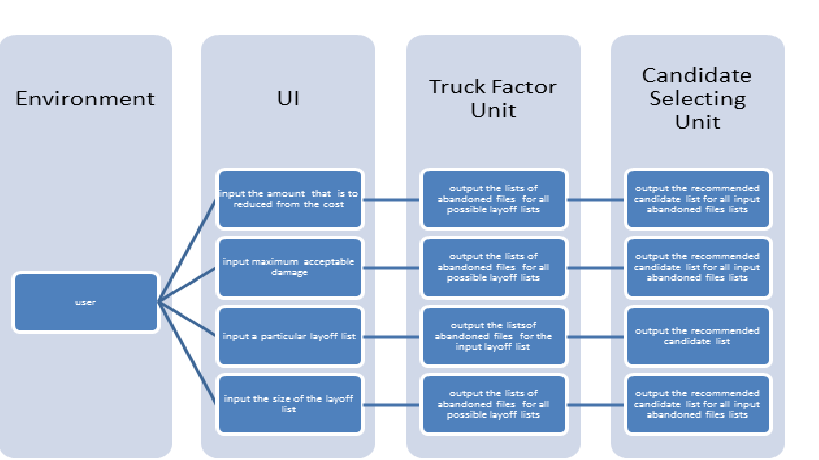
\includegraphics[scale=0.8]{structure}
	\label{structure}
\end{center}


\newpage
\section* {4. SCHEDULE}
\addcontentsline{toc}{chapter}{4. SCHEDULE}
Please check Table\ref{schedule} for the detail of the action schedule.
\begin{table*}[h]		
	\centering            
	\caption{Action Schedule}            
	\begin{tabular}{|c|c|}            
		\hline Number of Days required & Task   \\ \hline
		  2 & Select the programming language and the operating system \\ \hline
		  7 & recruit developers  \\ \hline
		  7 & develop the database building function  \\ \hline
          7 & implement the optimized truck factor algorithm  \\ \hline
          3 & develop the result output function \\ \hline
          1 & integrating test  \\ \hline
          7 & bugs fixing if any  (If no bugs, we don't need to do this task)\\ \hline
          7 & implement the successor candidate selecting algorithm \\ \hline
          1 & integrating test  \\ \hline
          7 & bugs fixing if any  (If no bugs, we don't need to do this task)\\ \hline
          7 & integrating all developed function unit and design UI  \\ \hline
          2 & final test \\ \hline
          7 & bugs fixing if any  (If no bugs, we don't need to do this task)\\ \hline
          1 & first release  \\ \hline
	\end{tabular}            
	\label{schedule}            
\end{table*}
\newpage
\section* {5. BUDGET}
\addcontentsline{toc}{chapter}{5. BUDGET}
Please check Table\ref{budget} for the detail of the project budget.
\begin{table*}[h]		
	\centering            
	\caption{Project Budget}            
	\begin{tabular}{|c|c|}            
		\hline Resource & Budget   \\ \hline
		2 programmers working 3 hours per day& \$7920 on total \\ \hline
        2 computers& \$2000 on total \\ \hline
        Total& \$9920  \\ \hline
	\end{tabular}            
	\label{budget}            
\end{table*}

\newpage
\section* {6. QUALIFICATIONS}
\addcontentsline{toc}{chapter}{6. QUALIFICATIONS}
\begin{center}
	
\includegraphics[scale=0.8]{cv_11.pdf}
	\label{structure}
\end{center}
%\section* {8. CONCLUSION}
%\addcontentsline{toc}{chapter}{8. CONCLUSION}
\newpage
\section* {7. PRESS RELEASE}
\addcontentsline{toc}{chapter}{7. PRESS RELEASE}

%\uppercase{Kickff helps reduce labor cost by providing a safe developer layoff solution for software companies.}
\subsection*{Concordia University,November 19, 2014}
A group of Concordia University students have developed a software application called Kickoff to help software companies control their labor cost. Based on the desired salary cut off amount, it can give out a programmer layoff list that is the least harmful to the software project and an abandoned source code take over solution.

Laying  off developer is dangerous to software companies. Since the part of project files maintained only by the layoff developers will become unknown to the company. If there was a bug reported in those files, nothing could be done until the remain developers learned how to maintain them. The learning process is time consuming, but the customer may select other product if the bug could not be fixed in a short time.  

However, In order to survive in a critical financial situation, software companies sometimes have to lay off developers to reduce the labor cost. Laying off senior developers cuts off more cost but lose more project files than laying off junior developers. Therefore deciding the layoff solution is difficult for software companies.

Kickoff first generates a set of possible solutions according to the target cutoff cost, then applies the "Optimized Truck Factor" algorithm to find out the least harmful solution and uses the "candidate finding system" to generate the project remedy solution. 

With Kickoff, it is easier for a software company to cut off their labor cost.  






\newpage
\section*{3. CONCLUSION}
\addcontentsline{toc}{chapter}{3. Conclusion}
It is harmful for a software project when there are some developers leaves. The damage is manifested as abandoned
files on the software system that can be difficult to maintain.
We believe that this damage can be reduced by finding experienced developers who have worked with the files that have co-changes with the abandoned files before to take over the abandoned files or to mentor new joiners to do so. Therefore we propose to apply the optimized truck factor algorithm to find out the abandoned files, and the candidate selecting algorithm to find out the experienced developers to build up the software Kickoff. With Kickoff, a software company can understand how harmful a particular layoff list is and how to reduce the damage. With Kickoff, a software company can also obtain information about all possible layoff solution by inputing the critical variable. Kickoff will be a very useful tool in software company management. In this proposal we've already scratched out the conceptual structure of it.


%%%%%%%%%%%%%%%%%%%%%%%%%%%%%%%%%%%%%%%%%%%%%%%%%%%%%%%
\backmatter
%%%%%%%%%%%%%%%%%%%%%%%%%%%%%%%%%%%%%%%%%%%%%%%%%%%%%%%

%\bibliographystyle{ieeetr}
\bibliographystyle{acm}
\bibliography{paper}


\appendix
%need to use \usepackage{amsmath,amssymb,amsthm,mathrsfs,amsfonts,dsfont}
\newpage
\section*{The Optimized TF Algorithm}
\addcontentsline{toc}{chapter}{Appendix A: The Optimized TF Algorithm }
The `truck factor' is a measure in the agile community of the number of developers that must leave (EX: get hit by a truck) before the project fails \cite{Torchiano2011Wetsom}. Previous work has calculated the maximum number of files
that are lost when a group of developers leave. Since this calculation has a
$O(n!)$, they are able to examine only small projects at one single point in time.
We contribute a stopping condition that allows us to calculate the maximum loss
quickly, so that we can examine the truck factor on large projects. We prove
that we attain the optimal solution and show how the truck factor for Chrome and
Linux changes over time. We compare the maximum loss to the actual loss that
Chrome and Linux have experienced suggesting how likely they are to suffer from
similar turnover events.

The naive TF algorithm proposed by Ricca et al \cite{Ricca2011PROFES} has a high time complexity.
When $n$ is the size of developer team and $m$ is the total number of files in the project then the time complexity is given by:
\begin{equation}T(n,m) = n*\sum_{i=1}^n \frac{n!}{i!(n-i)!}*m\end{equation}
For example, if a project has 30 developers then the number of developer combinations that is over 17 million.
In previous work, the largest project had only 38 developers
\cite{Torchiano2011Wetsom}. We are considering much larger projects, for
example, Chrome and Linux have 1000's of contributors. It is impractical to
combute all developer combination.
We introduce a stopping condition which we prove identifies, for a given group size, the set of developers who's loss will result in the maximum file loss.
\subsubsection{Truck factor definitions}
The following is the definition of symbols which will be used later:\\
$D =$ the set of all developers in the project.\\ %and $|D|$= the size of set $D$, in other words it is the total number of developers in the project.\\
$d_{i}=$ a particular developer in $D$, $i$ is the ID of the developer.\\
$F=$ the set of all files in the project.\\ %then $|F|$= total number of files in the project. \\
$f_{j}=$a particular file in $F$, $j$ is the ID of it.\\
$M(f_{j})=$ the set of developers who have modified the file $f_{j}$.\\
$I()$ is the logic function defined as:
\[ I(condition) = \left\{
\begin{array}{l l}
1 & \textmd{if condition is true}\\
0 & \textmd{otherwise}
\end{array} \right.\]
We first calculate the proportion of developer $d_{i}$ who have modified the file $f_{j}$ by equation:
\begin{equation}L(d_{i},f_{j})=\frac{1}{|M(f_{j})|} * I(d_{i} \in M(f_{j} )) \end{equation}
Then the file loss (FL) function returns how many files would be abandoned if a given developer combination $C$ left the project:
\begin{equation}
FL(C) = \sum_{d_i \in C} \sum_{f_i \in F} (I(M(f_i) \subseteq C)* L(d_i,f_i))
\end{equation}
Then the maximum file loss for a given group size is returned by the truck factor function:
$TF(C) = max(FL(C))$
We can see that a naive implementation of this algorithm will have a complexity of $O(n!)$, which is impractical to compute for large projects.
\subsubsection{Stopping Condition}
The shared proportion of the number of files a developer $d_i$ has modified on the project:
\begin{equation} L(d_i) = \sum_{f_i \in F} L(d_{i},f_{j}) \end{equation}
The upper bound of the file loss for a given developer combination $C$ is:
\begin{equation} UFL(C) = \sum_{d_i \in C}L(d_i) \end{equation}
Since \[\forall condition: I(condition) \leq 1 \]
We have:
\begin{equation} FL(C) \leq \sum_{d_i \in C} \sum_{f_i \in F} [1 * L(d_i,f_i)] = UFL(C)\end{equation}
%We have:
%\begin{equation}
%\forall C:FL(C)\leq UFL(C)
%\end{equation}
For each group size, we order the developer combinations by their $UFL$ value and calculate the $FL$ for each developer combination until the stopping condition, $UFL(C)<max(FL)$ is met.
In other words, we have shown that the number of files that a given group of developers modify, $UFL$, will be less than or equal to the number of files that these developers own exclusively, $FL$. Provided that we order the developers by the number of files that they modify, $UFL$, we can stop when the maximum loss that we calculated from the $FL$ function is greater than or equal to the total number of files that the subsequent group of developers modify. The algorithm is presented in Box?Algorithm
\subsubsection{TODO:combinations}
Unfortunately, we still must calculate must do $n!$ $UFL$ calculations. So we introduce a method to order these $UFL$ calculations.
TODO
\begin{algorithm}
	\SetAlgoLined
	\SetKwData{$d_i$}{$d_i$}\SetKwData{$F$}{$F$}
	\SetKwFunction{K}{K}\SetKwFunction{KL}{KL}\SetKwFunction{SF}{SF}
\end{algorithm}
\begin{raggedright}
	\scriptsize
	$TFX = threashold$,$i=1$;\\
	$F=$total number of files in the project;\\
	For each developer $d_i$ in the team $D$, calculate $K(d_i)$;\\
	Order $D$ by $K(d_i)$ decently;\\
	While $i\leq |D|$ repeat the block\{\\
	$Max\_fileLoss =0$;\\
	$combination\_generating(D,i)$;\\
	Initialize $input\_combination = input\_flow\_generating()$;\\
	While $SF(input\_combination)\geq Max\_fileLoss$ repeat the block\{\\
	If $KL(input\_combination) > Max\_fileLoss$ is true, $Max\_fileLoss=KL(input\_combination)$
	$input\_combination = input\_flow\_generating()$;\\
	\}\\
	out print: if you lost a developer combination of size $size$, your maximum file loss would be $Max\_fileLoss$;\\
	if $Max\_fileLoss \geq (TFX*F)$ is true the Truck Factor is $size$ and stop the algorithm;\\
	Otherwise increase $i$ by 1 and continue;\\
	\}\\
\end{raggedright}




\end{document}
